\documentclass[graphics,compress]{beamer}
\usepackage{graphicx} % Required for inserting images
\usepackage{minted}
\usepackage{tikz}
\usepackage{bbding} % For checkmark in itemize
\usepackage{hyperref}
\newcommand*\tick{\item[\Checkmark]}

% Adjustments to the page counts for the appendix
\newcommand{\backupbegin}{
   \newcounter{framenumberappendix}
   \setcounter{framenumberappendix}{\value{framenumber}}
}
\newcommand{\backupend}{
   \addtocounter{framenumberappendix}{-\value{framenumber}}
   \addtocounter{framenumber}{\value{framenumberappendix}} 
}

\hypersetup{
    unicode=false,          % non-Latin characters in Acrobat’s bookmarks
    pdftoolbar=true,        % show Acrobat’s toolbar?
    pdfmenubar=true,        % show Acrobat’s menu?
    pdffitwindow=false,     % window fit to page when opened
    pdfstartview={XYZ null null 1.00},    % disable zoom
    pdftitle={Enarx \& Steward Attestation},    % title
    pdfauthor={Richard Zak},     % author
    pdfsubject={Enarx's use of certificate signing requests for attestation},   % subject of the document
    pdfkeywords={Confidential Computing, EuroProofNet, Enarx, Cryptography}, % list of keywords
    pdfnewwindow=true,      % links in new PDF window
    %colorlinks=true,       % false: boxed links; true: colored links
    %linkcolor=red,          % color of internal links (change box color with linkbordercolor)
    citecolor=green,        % color of links to bibliography
    filecolor=magenta,      % color of file links
    urlcolor=cyan           % color of external links
}

\usetheme{Boadilla}
\title{Enarx \& Steward Attestation}
\author{Richard Zak // Enarx}
\date{28 March 2024}

\titlegraphic { 
\begin{tikzpicture}[overlay,remember picture]
\node[left=0.2cm] at (current page.-25){
    \href{https://enarx.dev}{
\includegraphics[width=1.1cm]{images/enarx.png}}
};
\node[right=1.0cm] at (current page.205){
    \href{https://www.linuxfoundation.org}{
\includegraphics[width=1.1cm]{images/LF.png}}
    \href{https://confidentialcomputing.io}{
\includegraphics[width=1cm]{images/ccc.png}}
};
\end{tikzpicture}
}

\begin{document}

\section*{Title}
\begin{frame}
\maketitle
\centering
\href{https://europroofnet.github.io/wg3-dresden24/}{EuroProofNet WG3, Dresden}
\vspace{2.2cm}
\end{frame}

\frame{\tableofcontents}

\section{Enarx}
\begin{frame}{What is Enarx?}
        Enarx:
        \begin{itemize}
        \item runs \href{https://webassembly.org}{WebAssembly} (\href{https://wasi.dev}{WASI}) applications in Trusted Execution Environments (TEEs) under Linux
        \begin{itemize}
        \item AMD \href{https://www.amd.com/de/developer/sev.html}{SEV}-SNP, Intel \href{https://www.intel.com/content/www/us/en/products/docs/accelerator-engines/software-guard-extensions.html}{SGX}/EDMM
        \item Others can be supported, like ARM \href{https://www.arm.com/architecture/security-features/arm-confidential-compute-architecture}{CCA}, etc.
        \end{itemize}
        \item has a very small TCB (Enarx + Wasmtime, your workload)
        \item is written in Rust
        \item can run on Windows, macOS, and ARM Linux without a TEE\footnote{Without protection, for testing \& development}
        \item open source project, Apache 2.0 licensed
        \end{itemize}
\end{frame}

\begin{frame}{WebAssembly}
    The use of \href{https://webassembly.org}{WebAssembly} System Interface (\href{https://wasi.dev}{WASI}) can be thought of as Posix for WebAssembly, and it provides some benefits for Enarx:
    \begin{itemize}
        \item Portability: The same binary works on different platforms (SGX or SNP, ARM or x86\_64, for example). The binary doesn't need to know, or care, which platform is in use.
        \item Flexibility: Programming language options, including C/C++, Go, Rust, Typescript, Ruby, Zig, others.
        \item Security: Wasi cannot open sockets or files, this has to be done on behalf of the WebAssembly runtime (Enarx uses \href{https://wasmtime.dev}{Wasmtime}), no possibility for unexpected network activity.
        \item Confidential Computing provides data privacy \& WebAssembly transforms the application into data, adding application privacy.
    \end{itemize}
\end{frame}

\section{Steward}
\begin{frame}{What is Steward?}
Steward is a Confidential Computing-aware Certificate Authority.
\begin{itemize}
    \item Written in Rust
    \item Apache 2.0 licensed
    \item Was a product of Profian, moved to the Enarx org on GitHub, donated to the Linux Foundation.
    \item Can be compiled as a native binary, or as a Wasi application for Enarx.
    \item Steward is stateless, only has the vendors' root CA certificates.
    \item Steward can generate a random key pair (for testing), or use provided public \& private key.
    \item Modular: can be expanded to support TDX, CCA, RISC-V, others.
    \item Doesn't require Enarx, just the expected Extension format.
    \item When workloads are deployed from Drawbridge, Steward adds workload hash to the Certificate (SAN field) as the Drawbridge URL\footnote{Was planned, might not be implemented.}.
\end{itemize}
\end{frame}

\section{Drawbridge}
\begin{frame}{What is Drawbridge?}
Drawbridge is a Confidential Computing-aware workload repository
\begin{itemize}
    \item Written in Rust
    \item Apache 2.0 licensed
    \item Was a product of Profian, moved to the Enarx org on GitHub, donated to the Linux Foundation
    \item Can be compiled as a native binary; in the future as a Wasi application for Enarx
    \item Only releases a workload to Enarx if it authenticates with Steward-signed certificate authentication.
    \item Workload data stored as a Merkle tree.
    \item Uses \href{https://openid.net}{OpenID} Connect to handle authentication through a provider.
\end{itemize}
\end{frame}

\section{Attestation via CSR}
\begin{frame}{Steward's Attestation Process}
Receive via HTTP Post a \href{https://en.wikipedia.org/wiki/Certificate_signing_request}{CSR} with an Extension:
\begin{itemize}
    \item Attestation report direct from the hardware.
    \item Vendor \href{https://en.wikipedia.org/wiki/Certificate_revocation_list}{CRL}
    \item AMD: CPU cert (Intel has the CPU cert in the Report)
    \item Intel: TCB report (firmware details) direct from Intel's API.
\end{itemize}

The following items are checked:
\begin{itemize}
    \item Does the attestation report signature match the CPU public key and report body?
    \item Is the CPU's certificate in the \href{https://en.wikipedia.org/wiki/Chain_of_trust}{PKI chain}?
    \begin{itemize}
        \item Vendor \href{https://en.wikipedia.org/wiki/Certificate_authority}{CA} $\rightarrow$ intermediate cert $\rightarrow$ CPU cert
    \end{itemize}
    \item Is the CRL signed by the vendor CA?
    \item Is the CPU's certificate not in the vendor CRL?
    \item Optional/configurable items:
    \begin{itemize}
        \item Minimum CPU firmware?
        \item Expected Enarx hash and/or signing key for the Enarx binary?
        \item Ensure Enarx hash and/or signing key isn't blacklisted.
    \end{itemize}
\end{itemize}

HTTP response: Signed cert or error
\end{frame}

\subsection{AMD}
\begin{frame}{AMD}
The AMD CSR Extension has a few additional items to check:
\begin{itemize}
    \item Ensure unused parts of the report are zeroed
    \item AMD has Policy Flags to check:
    \begin{itemize}
        \item Migration Assistant has to be disabled, we don't want Enarx losing control of it's guest.
        \item Debug is rejected if the Steward isn't compiled for debug mode, ensuring a release build won't allow a debug-enabled workload.
    \end{itemize}
    \item Hashes are SHA-384
\end{itemize}
\end{frame}

\subsection{Intel}
\begin{frame}{Intel}
The Intel Extension has additional checks:
\begin{itemize}
    \item The Intel TCB\footnote{Trusted Computing Base} report is sent as part of the CSR, and requires the ``fmspc''\footnote{Family-Model-Stepping-Platform Type-CustomSKU}, which identifies the hardware, and checks:
    \begin{itemize}
        \item Whether the firmware is updated, or Intel advisories for the firmware.
        \item Signing certificate \& signature of the TCB.
        \item TCB signing certificate is part of Intel's PKI chain.
        \item Next update date for the TCB hasn't passed.
        \item The signature is valid.
    \end{itemize}
    \item Steward checks that the FMSPC from the public key matches the TCB report.
    \item Hashes are SHA-256
\end{itemize}
\end{frame}

\subsection{Example Config}
\begin{frame}[fragile]{Example Config}
    \begin{minted}[fontsize=\scriptsize]{toml}
[sgx]
signer = ["7a49a07df0f8e90a6e1d9a63e3c696d9c844f0e3f8739b21daa640f99facc48a"]
hash = ["4046ea255f0455131a024e1265ac1ebd131fdbd1240f1712a00381f6f04e8c15"]
features = ["Debug", "ProvisioningKey", "EInitKey", "KSS"]
enclave_security_version = 0 # isv_svn
enclave_product_id = 0 # isv_prodid
allowed_advisories = ["INTEL-SA-00289", "INTEL-SA-00381", "INTEL-SA-00389",
    "INTEL-SA-00477", "INTEL-SA-00586", "INTEL-SA-00614", "INTEL-SA-00615",
    "INTEL-SA-00617", "INTEL-SA-00657"]

[snp]
signer = ["7dc22240a8344fce6ba5f22ffbedabc52d4123ae0ba1c59796e521b953916b503f223b15c4429e7d8c5489ad71f1e193"]
id_key_digest = ["d71a4d1da440d515cd69fbb1314acf4221726e82768a8bf6e4a4063ed542ac78349c8145b4666a4242a91a374387b473"]
hash = ["ff717ae719840c93c1fca3b7db96488454c3c21b43531488eecff51cfed3febcd91da8be87a4cbcbc52a3bae770987c3"]
abi = ">=1.51" # firmware version, SemVer
policy_flags = ["SMT"]
platform_info_flags = "SME"
    \end{minted}
\end{frame}

\section{Workflow}
\begin{frame}{Workflow}
    \only<1> {
        \begin{enumerate}
            \item Administrator deploys an application from Drawbridge by name \& hash
            \item Enarx contacts Drawbridge and gets the URL of the Steward
            \item Enarx gets the hash of the intended workload
            \item Enarx creates an empty Keep (Enarx without workload)
            \item Enarx asks the CPU for an attestation report with workload hash
            \item Enarx generates a private key, CSR, adds the attestation report to the CSR as an Extension
            \item Enarx sends the CSR to Steward
            \item Steward validates the CSR and responds with a signed certificate
            \item Enarx authenticates to the Drawbridge and fetches workload
            \item Drawbridge ensures the Enarx cert is in the Steward's PKI chain
            \item Drawbridge responds with the workload back to Enarx
            \item Enarx ensures the workload's hash matches the expected hash (\#1)
            \item Application runs, using Steward-signed certificate for communicating with third parties
        \end{enumerate}
    }
    \only<2> {
        \centering
        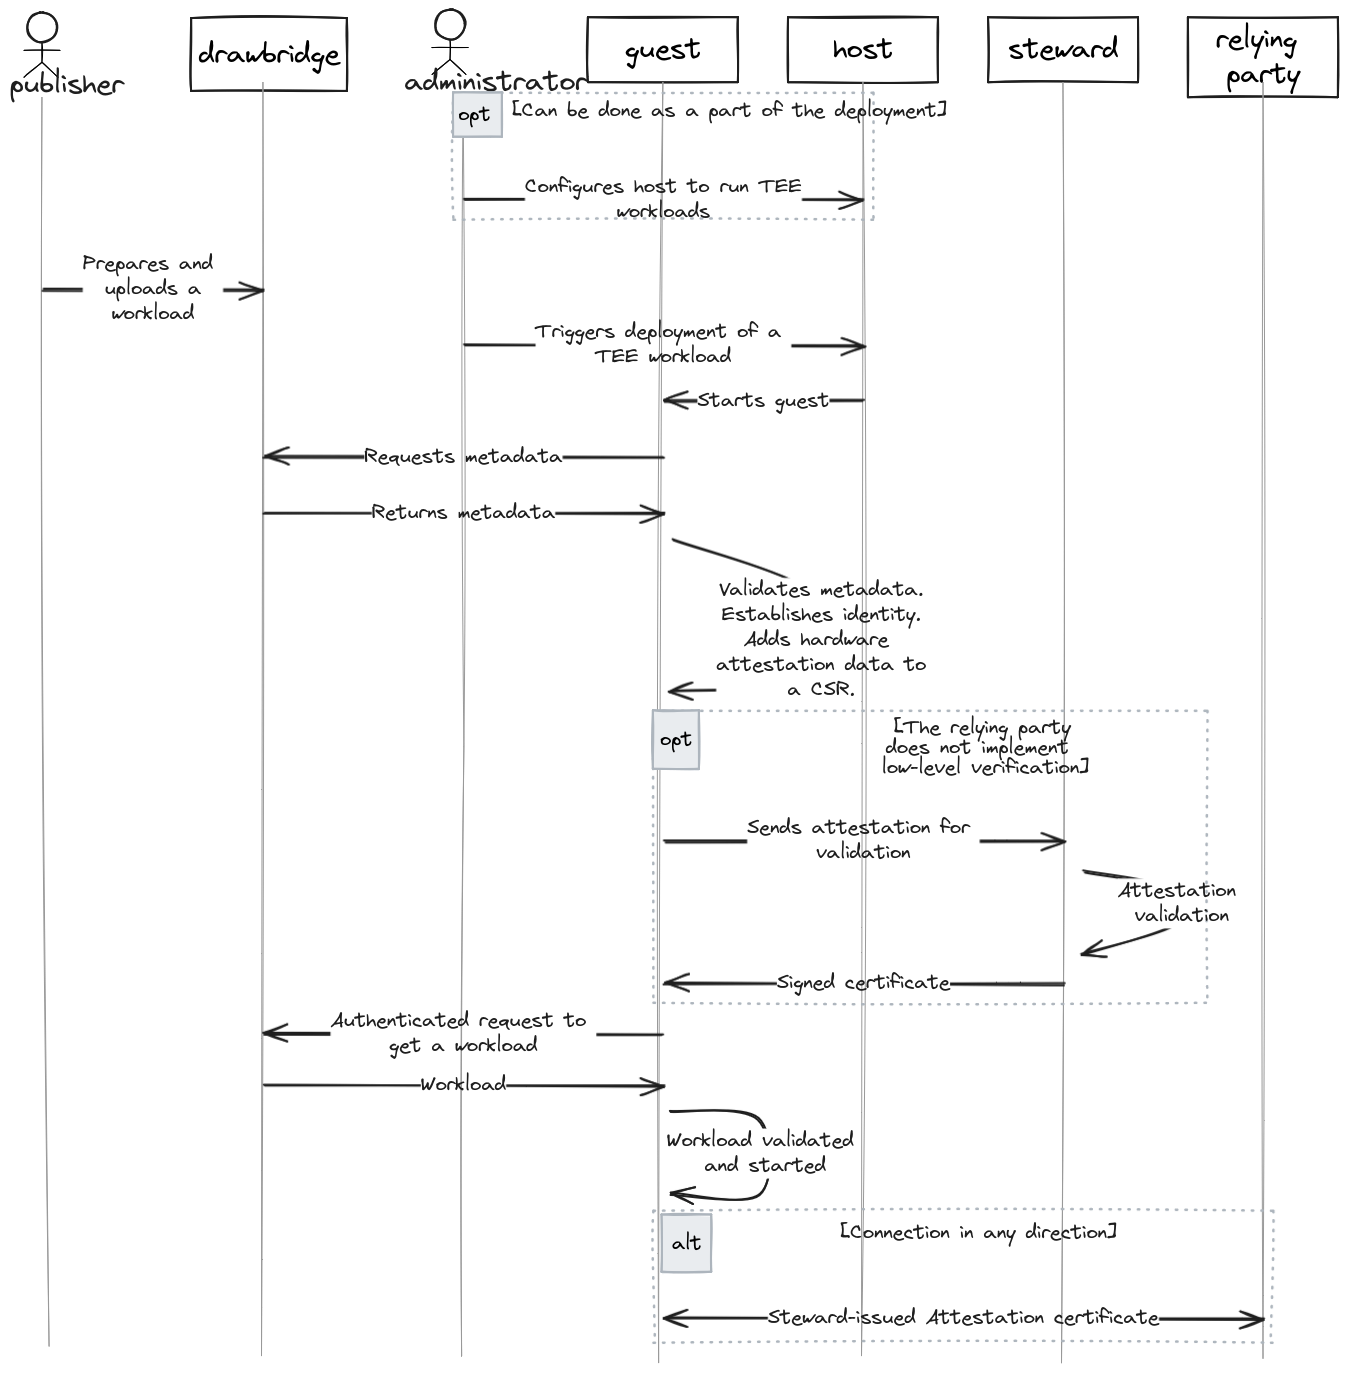
\includegraphics[width=1.01\linewidth,height=0.71\linewidth]{images/attestation-flow-excalidraw.png}
    }
\end{frame}

\section{Merits of CSR}
\begin{frame}{Merits of Attestation via CSR}
\begin{itemize}
    \item CSRs \& Certs don't require special software on the client end, replying parties can use existing software.
    \begin{itemize}
        \item No new protocol required.
        \item No special data format to be processed by relying party.
    \end{itemize}
    \item No private information about the hardware is leaked.
    \item Attest once, get a token (cert) which can be used in various ways without having to re-evaluate.
\end{itemize}
\end{frame}

\section{Drawbacks of CSR}
\begin{frame}{Drawbacks of Attestation via CSR}
The Steward CA has to be trusted:
\begin{itemize}
    \item added the Steward CA to the operating system's list of CAs, or modify the 2\textsuperscript{nd} party application to only allow this specific CA;
    \item any configuration of the Steward isn't known to the relying party:
    \begin{itemize}
        \item any allowed vulnerabilities in the firmware?
        \item allowed versions of Enarx?
        \item how to address configuration with non-Enarx-based attestation?
    \end{itemize}
\end{itemize}
\end{frame}

\section{Acknowledgements}
\begin{frame}{Acknowledgements}
Many thanks to:
\begin{itemize}
    \item \href{https://github.com/npmccallum}{Nathaniel McCallum} \& \href{https://github.com/MikeCamel}{Mike Bursell} for going out on a limb and creating Enarx, creating Profian, and hiring me;
    \item \href{https://github.com/haraldh}{Harald Hoyer} \& \href{https://github.com/rvolosatovs}{Roman Volosatovs} for their patient mentorship;
    \item \href{https://github.com/nickvidal/}{Nick Vidal} for continuing to help Enarx as the Community Manager;
    \item EuroProofNet for having me;
    \item AMD and Intel for their exceptional technologies and fantastic documentation; and
    \item the Confidential Computing Consortium for supporting this technology and sending me.
\end{itemize}
\end{frame}

\appendix
\backupbegin
\section{Appendix}
\begin{frame}{The Future of Enarx}
    \only<1> {
        Enarx development has slowed since Profian closed, but it's alive and there are a few things on the roadmap:
        \begin{itemize}
            \item Recreate \texttt{try.enarx.dev}, where people can run their application in a hosted TEE for a limited time using Profian's ``Benefice'' project.
            \item Run a public Steward for people to test Enarx with an Enarx CA.
            \begin{itemize}
                \item Possibly run a demo or debug Steward with looser restrictions.
                \item URL: \texttt{ca.enarx.dev}
                \item HSM integration (need to buy \& learn how to use an HSM)
            \end{itemize}
            \item Run a public Drawbridge.
            \item Continue work on the VFS project for Enarx:
            \begin{itemize}
                \item Network connection policies
                \item Read-only on the host unencrypted
                \item Transparently encrypt writes to local disk.
                \item Virtual file operating for managing crypto operations.
                \item Virtual file operations for opening new network connections
            \end{itemize}
            \item Continue to promote Enarx online and in-person.
            \item Keep Enarx updated with changes in WebAssembly.
        \end{itemize}
    }
    \only<2> {
        Accomplished post-Profian:
        \begin{itemize}
            \tick Received \& configured CI servers so Enarx commits are again tested with SGX \& SNP.
            \tick Merged in support for AMD SNP v10 patches (thanks \href{https://github.com/Freax13}{Tom Dohrmann}!)
            \tick Steward \& Drawbridge relicensed, moved to Enarx org.
            \tick Keeping the projects' dependencies updated (in progress).
            \tick Keeping Enarx's dependency crates\footnote{Ciborium, Crt0stack, Flagset, Sgx, Vdso, etc} created by Enarx/Profian updated and providing releases (on-going).
            \tick Updates and content for the website (on-going).
            \tick Gain control of social media accounts (Mastodon, LinkedIn) for Enarx.
        \end{itemize}
    }
\end{frame}

\begin{frame}{Attestation Workflow Mermaid}
    \centering
    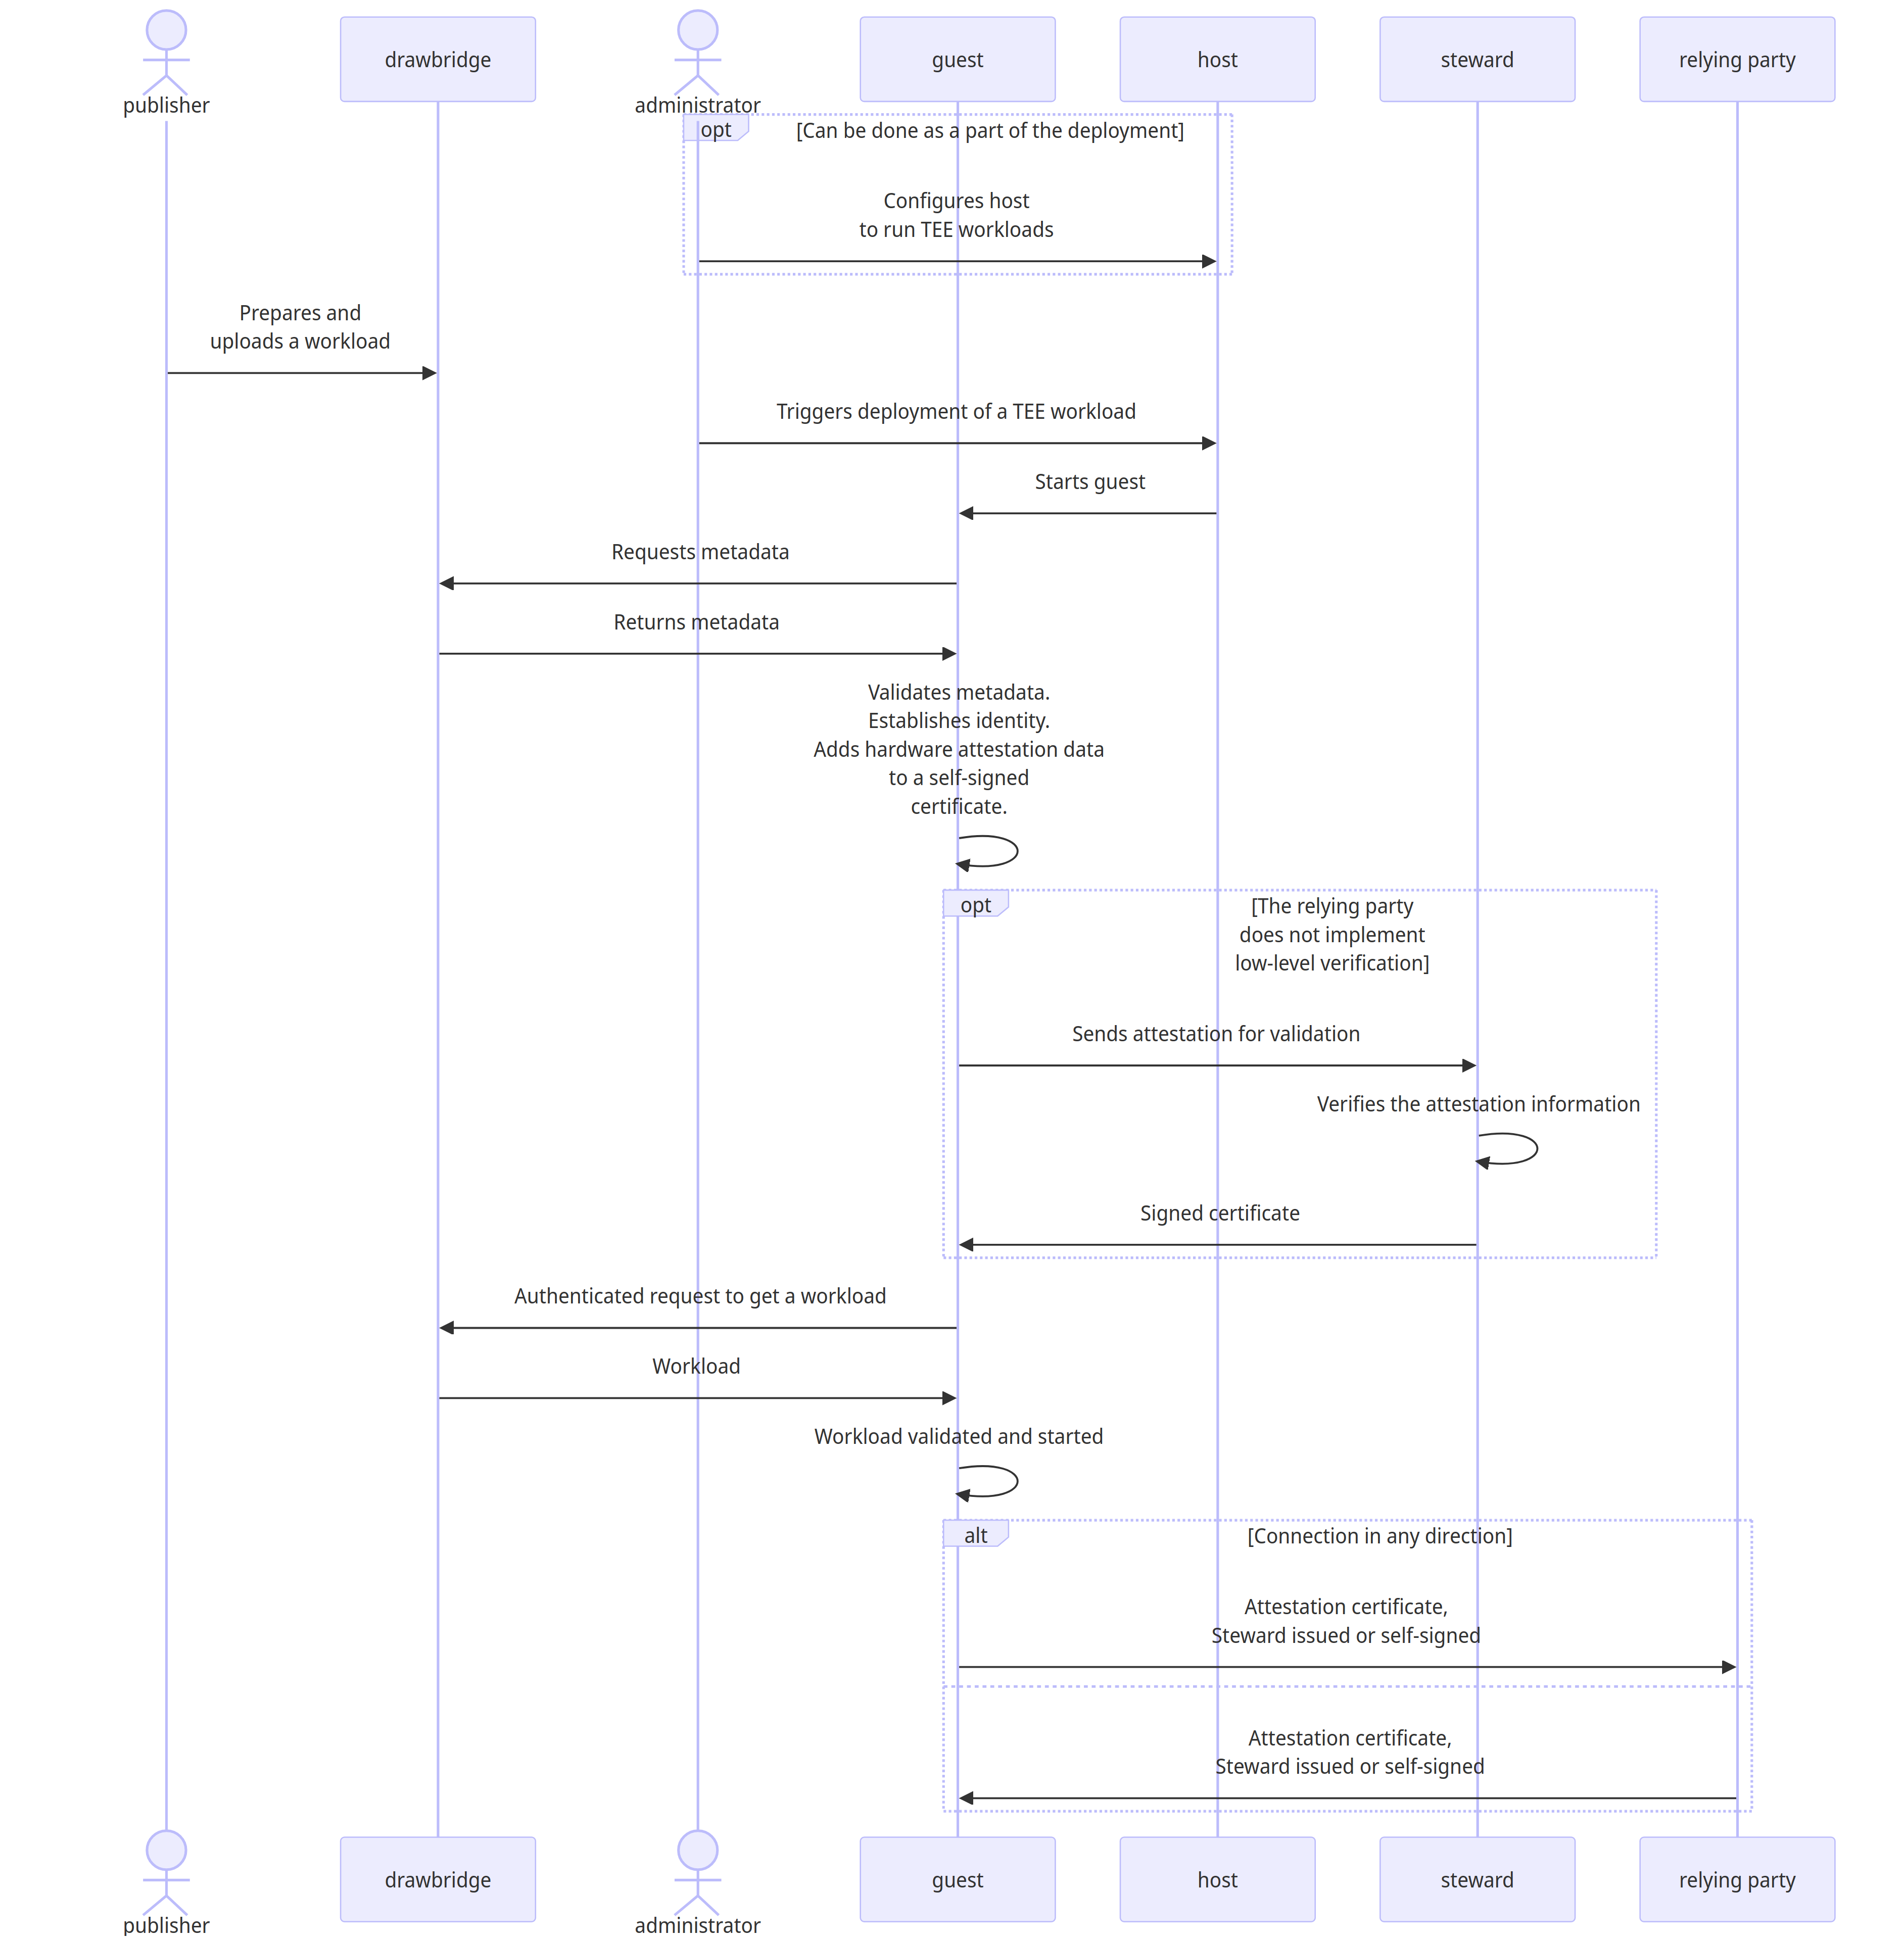
\includegraphics[width=1.01\linewidth,height=0.71\linewidth]{images/attestation-flow-mermaid.png}
\end{frame}
\backupend

\end{document}
